On first sight the key findings discussed by Frantz and 
Kendall-Taylor hold. However, critical evaluation of key
statistical assumptions, predictive accuracy and model
parsimony give reason to doubt their statistical adequacy 
and substantial significance. Following a brief recapitulation of the key results each point is briefly discussed in the remainder of this section.

\begin{figure}[!ht]
  \centering
  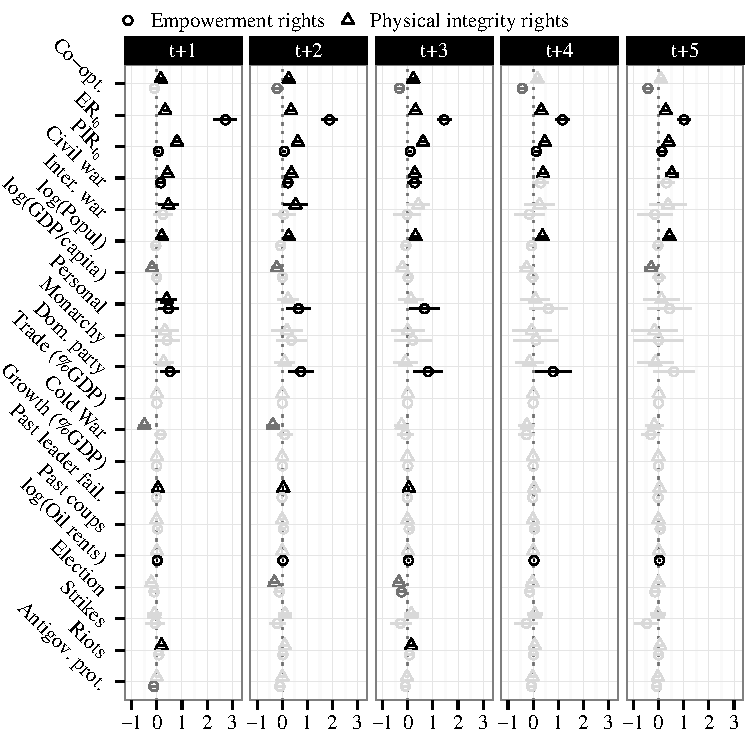
\includegraphics[width=\linewidth]{./sections/03replication/coefPlotOriginal.pdf}
  \caption{How co-optation affects political repression.
    Confidence intervals at the .95 level, positive 
    coefficients black, negative estimates grey, statistically
    insignificant results faded. Cubic polynomials and 
    cut points not shown.%
  }
  \label{fig:coefPlot}
\end{figure}

Figure \ref{fig:coefPlot} summarizes all ordered logistic
regressions presented in the original publication. 
Differences between the published and the replicated 
analyses are often negligible. With few exceptions 
coefficients and cluster robust standard errors 
agree up to two decimal places.\footnote{A fundamental
difference concerns the polynomials on tenure duration. 
The original models would not converge in $R$ unless 
multicollinearity was reduced by using orthogonal 
polynomials.} As can be seen from the top row in 
Figure \ref{fig:coefPlot} higher levels of co-optation 
concur with lower levels of empowerment rights 
restrictions, but they tend to go hand in hand with 
increases in physical integrity violations. Moreover, in 
line with the idea of inert government practices the 
attenuating impact of co-optation on empowerment rights 
restrictions increases in absolute size when moving from
$t+1$ to $t+5$. The same time-dependent dynamic is not 
observable for physical integrity violations. Finally, all 
models speak to the staying power of political repression 
because all lagged responses are positively signed and
statistically significant.\footnote{Why 
Erica Frantz and Andrea Kendall-Taylor regard all lagged 
reponses as continuous and treat all leads as ordinal 
variables is not clear from the paper.} In short, all
key findings can be reproduced and a more detailed discussion of the original publication is possible.

\begin{table}[!htb]
\centering
\caption{Parallel-regressions assumption: $\chi^2$-comparisons}
\label{tbl:Chi2comparisons}
  \begin{tabular}{ll*{5}{c}} \toprule
    ~ & ~ & $t+1$ & $t+2$ & $t+3$ & $t+4$ & $t+5$ \\ \cmidrule{2-7}
    \multirow{2}{*}{Empowerment rights} & Unadj. P-value & 1.000 & 0.499 & 0.000 & 0.000 & 0.000 \\
    ~ & Bonf. adj. P-value & 1.000 & 0.833 & 0.000 & 0.000 & 0.000 \\
    \multirow{2}{*}{Physical integrity} & Unadj. P-value & 0.003 & 0.002 & 0.000 & 0.000 & 0.000 \\
    ~ & Bonf. adj. P-value & 0.077 & 0.052 & 0.001 & 0.000 & 0.000 \\ 
    \bottomrule
    \multicolumn{7}{l}{\textit{Note:} P-values were averaged over all imputed models.} \\
  \end{tabular}
\end{table}

\begin{wrapfigure}{r}{0.45\textwidth}
\centering
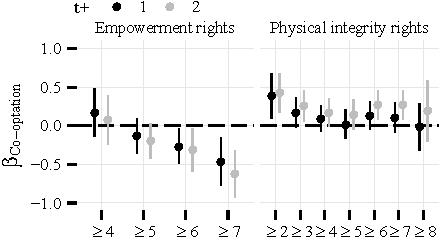
\includegraphics[width=\linewidth]{./sections/03replication/parallelRegressionsCoefPlot_manualLabels.pdf}
\caption{Separate logistic regressions results. Confidence
  intervals at the .95 level added.}
\label{fig:separateLogisticCoef}
\end{wrapfigure}
Ordered logistic regression models rest on the 
parallel-regressions assumption. They constrain differences 
between the cumulative distribution functions of any two 
categories to a a constant \citep[476]{Fox.2008}. In other 
the words, the slope of those curves must not change
and hence all regression coefficients are constrained to 
equality between any two categories. One way to test this
assumption is a $\chi^2$-comparison between the constrained 
coefficients and their unconstrained alternatives from a 
multinomial regression. As shown in Table 
\ref{tbl:Chi2comparisons} only the four models 
predicting political repression at $t+1$ and $t+2$ 
withstand this test and reject the alternative hypothesis 
of non-constant coefficients and thus support the choice of
statistical model. However, since the null hypothesis is 
saved only by very conservative Bonferroni adjusted 
P-values a closer look at the four supported
models seems justified. To that end $j-1$ separate logistic 
regressions are fit to the set of binary responses 
$\mathbbm{1}_y(y_{i} \ge j)$.\footnote{As the marginal 
categories of all response variables are sparsely populated
(c.f. Figure \ref{fig:scatterRepression}) perfect
separation occurred on several instances. The affected 
response levels were dropped from Figure \ref{fig:separateLogisticCoef}.} If the parallel-regressions assumption holds
the coefficients should differ little as $j$ increases. 
Figure \ref{fig:separateLogisticCoef} shows the results for 
the key regressor co-optation. While the right-hand panel 
raises little reason for concern, coefficients in the 
left-hand panel exhibit a clear trend. As the level of 
empowerment rights restrictions increases co-optation 
develops more of a punch. In sum, the majority of models 
fails the parallel-regressions assumption and even 
if it is not rejected outright the published analyses give 
reason for concern.